% !TeX root = ../main.tex

\chapter{绪论}\label{chap:intro}

人工智能是指通过电子信息技术呈现出人类智能的技术,作为一门新兴前沿学科,它的发展正在深深地影响着社会的进步和人类的发展。目前世界各国都在大力发展人工智能技术,众多科研人员投身于最前沿的技术研究中。尽管我国也正在为建设世界一流的人工智能强国而努力,但不可否认的是在软件硬件等多个层面上均和国际领先国家存在一定差距。为了弥补这一差距,我们必须抓住21世纪新的机遇,顺应时代的发展,在科技进步的浪潮之中争当中流砥柱。本课题以人工智能领域中的强化学习方法为主要研究背景,对其在现实世界中的实际应用价值展开具体分析。本章内容主要从以下方面进行具体阐述:

\begin{itemize}
    \item 研究背景与意义
    \item 本文的主要内容
    \item 本文的组织结构
\end{itemize}

\section{研究背景与意义}

机器学习作为人工智能领域内的一个核心支撑工具,主要由区分为监督学习和无监督学习组成\cite{sathya2013comparison,goodfellow2016deep}。监督学习是提供数据与对应标签的数据集并学习数据间关联结构的算法,无监督学习则是由无显式关联结构的数据集推导数据样本间关联结构的算法\cite{bishop2006pattern}。除了上述介绍的两类算法,在机器学习领域内还存在一类隐式提供数据标签的弱监督算法\cite{zhou2018brief},强化学习便是弱监督算法中的一类重要算法。在强化学习中,训练数据是由智能体与环境交互生成并进行自我探索学习,智能体在给定的奖励反馈引导下,最终学习策略做出最优决策,产生最大收益\cite{tan1993multi}。在这个自我探索的学习过程中,智能体并不会被具体引导,而是大量与环境交互进行探索和试错,根据历史经验和未来预测去发现能产生高价值的收益最优行为 \cite{kaelbling1996reinforcement,sutton2018reinforcement}。强化学习因其简单通用的算法框架,被认为是最能胜任通用人工智能问题的解决方案\cite{shoham2003multi}。 

目前,强化学习在包括游戏,广告,推荐,对话系统,机器人等多个领域均展开了广泛的应用\cite{cai2017real,wang2018reinforcement,li2016deep,riedmiller2009reinforcement}。代表性的工作为DeepMind公司开发的AlphaGo围棋AI \cite{chen2016evolution},如图~\ref{fig:rl-go}~所示,强化学习算法可以根据棋盘状态信息,预测对手未来的轨迹,并基于预测信息做出最合理的决策\cite{holcomb2018overview}。但在更加复杂的真实场景中,由于强化学习算法需要大量与环境和传感器、控制器等设备进行数据交互,并且实时采集环境数据、发送策略指令,而这些硬件设备在各种工作场景中效率低下,远不如计算机处理器芯片的高效性能,同时设备损耗带来的成本高昂,导致强化学习算法会受限于这些硬件设备的工作效率\cite{zhang2021robust,yao2021sample},使得强化学习算法的样本利用效率成为其应用于真实场景的关键瓶颈之一\cite{arulkumaran2017deep,kober2013reinforcement}。此外,由于强化学习算法往往以平均收益为优化目标,尽管能在期望意义下取得整体的最大收益,但是在个别极端情况下可能产生较大损失,这也是强化学习算法学习策略产生不稳定性和不安全性的主要原因。安全性的缺乏导致强化学习算法也不被自动驾驶等一些高安全性要求的应用领域接受\cite{ling2015application,cheng2019end,zhang2020cautious}。

\begin{figure}
  \centering
  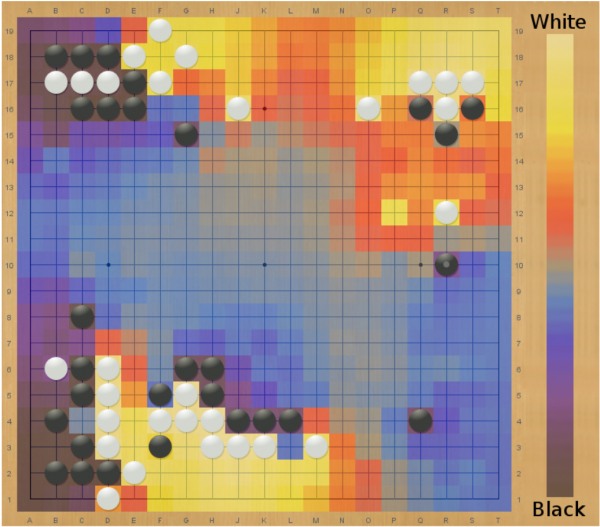
\includegraphics[width=0.8\linewidth]{figures/rl-go.png}
  \caption{强化学习算法在棋类游戏中的应用}
  \label{fig:rl-go}
\end{figure}


传统的无模型强化学习在训练阶段往往需要和任务环境进行上千万次的交互和数据采样才能收敛学习出决策策略 \cite{degris2012model},这样的样本数量级在虚拟环境下是完全可行的,而在现实问题中,收集上千万条交互数据的成本过于高昂,因此传统的无模型强化学习算法极难应用在现实任务场景中。在现有的工作中,基于模型的强化学习被广泛应用于解决上述的样本效率问题\cite{osband2014model,moerland2020model}。相较于无模型强化学习,基于模型的强化学习算法首先将收集的交互数据$(s_t,a_t,r_t,s_{t+1},a_{t+1},r_{t+1},\ldots)$作为有标签的训练数据集,通过监督学习的方式学习得到环境的近似模型$\mathcal{M}$,再由策略与该模拟环境交互,生成模拟的预测轨迹,即$s_{t+1}=\mathcal{M}(s_t,a_t)$。基于模型的强化学习主要可以根据如何使用所学的环境模型而分为以下3个类别\cite{pal2020brief}:

\begin{enumerate}[1)]
    \item 作为新的数据源:通过与环境模型交互产生数据,作为额外的训练数据源来补充算法的训练。
    \item 增加决策的上下文信息:在进行状态价值的估计时,通过与环境模型进行交互,交互过程中的上下文信息提供给算法来帮助其决策。
    \item 增加状态价值估计的准确性:在进行状态价值估计时候,基于环境模型来展开一定步数,然后辅助无模型强化学习算法,给出一个更准确的状态价值估计,加速算法收敛。
\end{enumerate}

除了样本利用效率问题,在强化学习领域内,所学策略的稳定性和安全性问题也是影响其实际应用的关键瓶颈之一\cite{junges2016safety}。在强化学习任务中,算法的主要目标是使长期收益最大化,虽然能使收益的期望值最大化,但期望的最大值并不意味着整体意义上的稳定性,即使个别情况较小的低收益,也对整体的期望影响不大,因此在最大化期望收益时,这些偶尔发生的低收益状态会被忽视掉,往往容易导致策略过于追求收益,却忽视整体上的安全性和稳定性 \cite{garcia2015comprehensive,xiong2016combining}。尽管在普通的任务或者仿真环境中,一些偶尔发生的决策失误并不会带来太大的损失,使得算法常常忽视这些场景,但若要部署到真实环境中,例如在昂贵的机器人平台,一些不稳定的策略容易使机器人受损 \cite{kormushev2010robot};在农业自动化任务中,一般的强化学习算法策略常常导致农作物突发坏死 \cite{bu2019smart};而在自动驾驶任务中,未经安全性优化的策略有可能导致危险的事故 \cite{sallab2017deep,ferdowsi2018robust}。

作为一种缺乏可解释性的决策算法,强化学习训练得到的“黑箱”策略很难再加入人类的先验知识作为指导\cite{mousavi2020black,wei2021non}。由于其不可靠性,强化学习一直不被认可用于真实环境的应用中\cite{berkenkamp2017safe,jin2020stability}。但最近一些研究强化学习的安全性的工作为这一难题提供了突破口,主要可以分为3个类别 \cite{munos2016safe}:

\begin{enumerate}[1)]
    \item 降低训练方差:过高的方差往往意味着策略的不稳定性,导致在决策使做出一些意料之外的危险动作。在一些工作中,通过将收益方差作为风险指标进行优化,从而提升策略的安全性;
    \item 关注最坏情况:与上面类似地,通过增加对最坏情况的关注度,着重训练这样的高风险状态,使得策略能够合理地处理这些极端情况;
    \item 主动惩罚错误:通过将错误状态出现的次数或概率作为惩罚项进行训练,最终所得策略能够一定程度上规避这些高风险状态,同样提升了安全性。
\end{enumerate}

\section{本文的主要内容}

\begin{figure}[t]
  \centering
  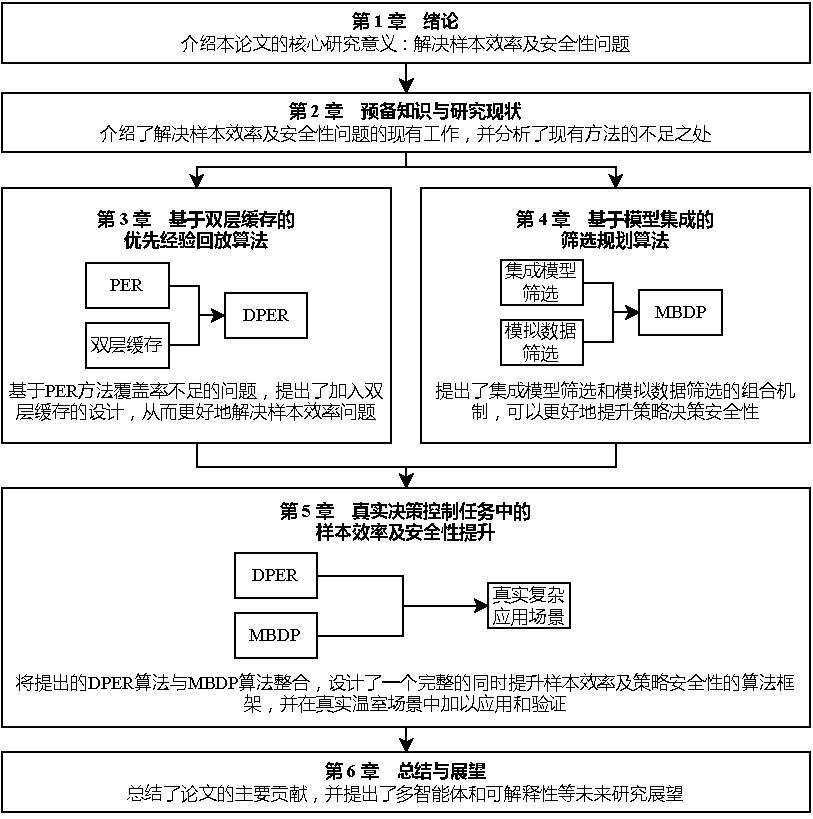
\includegraphics[width=0.8\linewidth]{figures/paper-struc.pdf}
  \caption{论文章节内容与关系结构}
  \label{fig:paper-struc}
\end{figure}

本论文介绍了强化学习算法中样本利用效率和策略安全性的意义和背景,详细阐述了强化学习中的基本概念和框架,以及相关研究领域中的研究现状,进而研究和分析了现有强化学习算法在样本利用效率和策略安全性上的不足之处,从经验回放和样本筛选两个角度分别设计了有效的解决方案,并在理论和实验上都验证了解决方案的有效性和可行性。

针对强化学习的样本利用效率问题,本文首先提出了基于双层缓存的优先经验回放算法(Double-layer Prioritized Experience Replay,DPER)。DPER算法设计了一种双层经验回放池,能够在额外的第二层经验回放池中长时缓存全局空间的经验回放样本,提高了经验回放样本在样本空间中的有效覆盖率,加快了策略学习的收敛速度,从而实现了对算法样本利用效率的提升。

针对强化学习的策略安全性问题,本文又进一步提出了基于模型集成的筛选规划算法(Model-Based Dropout Planning,MBDP)。MBDP算法由集成模型筛选模块和模拟数据筛选模块组合而成,其中集成模型筛选模块通过计算集成模型中单个模型的预测精确度来进行优先级筛选,其主要作用是以少量鲁棒性下降的代价对算法整体起到样本利用效率的提升;而模拟数据模块则是对生成的模拟样本计算收益值来进行优先级筛选,其主要作用是以少量样本效率下降的代价对算法整体起到鲁棒性的提升。两个模块在对抗的作用下最终起到了兼顾样本效率提升和鲁棒性提升的效果,其所学习得到的决策策略在保障样本效率的前提下,通过更优秀的鲁棒性来实现决策策略安全性的提升。

本文随后在Cliff-Walking环境和OpenAI-Gym提供的Mujoco环境下进行了模拟仿真实验,对所设计的DPER算法和MBDP算法进行了实验验证。实验结果证明了所设计的基于双层缓存的优先经验回放算法中所提出的双层经验回放池能够有效地增强策略学习的收敛速度,相比优先经验算法有更好的样本利用效率。而基于模型集成的筛选规划算法也在Mujoco中多个仿真环境下的实验中验证了其样本利用效率和鲁棒性的同时提升。为了进一步验证所提出的算法在真实应用场景中的安全性提升效果,本文以基于模型集成的筛选规划算法为核心,以自动化温室决策控制为任务目标,设计了温室自动化控制策略学习算法,并在仿真模拟器及真实环境中进行了验证实验。结果表明,算法不仅相比于基线方法有着更好的收敛性能,还表现出了超越人类平均水平的决策性能。与此同时,算法在受环境干扰的情况下还表现出优异的稳定性,能够大幅提升自动化温室决策策略的安全性。这一实验结果也进一步地证明了本文所设计的算法能够在强化学习算法中有效提升样本利用效率和安全性。

本论文的研究工作具体的创新点和贡献可概括如下:

\begin{enumerate}[1)]
    \item 提出了通过双层经验回放池进行不同速率优先级经验回放的强化学习算法,实现了更大的样本空间经验回放覆盖率,有效提升了强化学习算法的样本利用效率;
    \item 提出了基于集成模型预测精确度筛选和基于模拟数据样本反馈值筛选的双重筛选规划算法,实现了在保证样本利用效率的前提下对所学决策策略安全性进行有效提升;
    \item 在多种仿真和真实实验环境中对所提出的算法进行了实验评估,验证了算法在样本利用效率和策略安全性上的提升效果。
\end{enumerate}

\section{本文的组织结构}

本文的组织结构如下:第~\ref{chap:intro}~章是绪论部分,主要介绍了强化学习的基本背景和强化学习算法中样本利用效率及策略安全性的研究意义;第~\ref{chap:background}~章为预备知识与研究现状,通过大量调研学术文献,详细介绍了强化学习的基本概念、求解最优决策策略的方法框架和针对所要研究的样本效率问题及安全性问题的研究现状;第~\ref{chap:dper}~章详细介绍了基于双层缓存的优先经验回放算法,具体描述了该算法的设计思路和实现细节,并分析了验证实验中的结果;第~\ref{chap:mbdp}~章详细介绍了基于模型集成的筛选规划算法,阐述了算法的设计灵感和细节,通过理论分析论证了算法的有效性和合理性,并进一步根据实验结果加以验证;第~\ref{chap:greenhouse}~章将所设计的算法应用于真实的复杂场景中,设计了自动化温室决策控制任务背景下的强化学习算法框架,通过更苛刻的真实条件验证了算法的有效性;第~\ref{chap:summary}~章对全文进行了总结,分析了本论文工作中存在的不足之处,并对未来的工作进行了思考和展望。